% Created 2023-10-05 Thu 12:38
% Intended LaTeX compiler: pdflatex
\documentclass[11pt]{article}
\usepackage[utf8]{inputenc}
\usepackage[T1]{fontenc}
\usepackage{graphicx}
\usepackage{longtable}
\usepackage{wrapfig}
\usepackage{rotating}
\usepackage[normalem]{ulem}
\usepackage{amsmath}
\usepackage{amssymb}
\usepackage{capt-of}
\usepackage{hyperref}
\usepackage{alltt}
\usepackage[utf8]{inputenc}
\usepackage{mdwlist}
\usepackage{amssymb}
\usepackage[fleqn]{mathtools}
\usepackage{multicol}
\usepackage{enumitem}
\usepackage[dvipsnames]{xcolor}
\usepackage{wrapfig}
\usepackage{array}
\usepackage{nccmath}
\usepackage{graphicx}
\usepackage{fancyhdr}
\usepackage{tikz}
\usepackage[margin=0.5in]{geometry}
\usepackage{fdsymbol}
\pgfdeclarelayer{background}
\pgfdeclarelayer{foreground}
\pgfsetlayers{background,main,foreground}
\newcommand{\done}{$\quad\blacksquare$}
\newcommand{\lSeq}[1]{\left\{#1_n\right\}^{\infty}_{n=1}}
\newcommand{\lHed}[1]{\noindent\textbf{#1}}
\newcommand{\0}{\emptyset}
\newcommand{\N}{\mathbb{N}}
\newcommand{\Z}{\mathbb{Z}}
\newcommand{\Q}{\mathbb{Q}}
\newcommand{\R}{\mathbb{R}}
\newcommand{\C}{\mathbb{C}}
\newcommand{\lcm}{\text{lcm}}
\newcommand{\Unif}{\text{Unif}}
\newcommand{\Ber}{\text{Ber}}
\newcommand{\Binom}{\text{Binom}}
\newcommand{\Pois}{\text{Pois}}
\DeclareMathOperator{\proj}{proj}
\DeclareMathOperator{\vspan}{span}
\DeclareMathOperator{\Log}{Log}
\DeclareMathOperator*{\Res}{Res}
\date{}
\title{Analysis I}
\hypersetup{
 pdfauthor={},
 pdftitle={Analysis I},
 pdfkeywords={},
 pdfsubject={},
 pdfcreator={Emacs 29.1 (Org mode 9.7)}, 
 pdflang={English}}
\begin{document}

\maketitle
\section*{October 2, 2023}
\label{sec:org58c1467}
\subsection*{Lecture Notes}
\label{sec:org27a14e4}
Class will not have dedicated lecture notes. Many are available already.\\[0pt]
Undergraduate notes are available on Canvas.\\[0pt]
Lecture 1 overview available on Canvas (lecture1.pdf).\\[0pt]
\subsection*{Tentative Office Hours}
\label{sec:org39ab572}
Mondays 2-3pm and Tuesday 1-2pm.\\[0pt]
\subsection*{Homework}
\label{sec:org618a88a}
Nominally due at beginning of class; ask for leeway if needed.\\[0pt]
First week homework will be review of undergraduate proofs.\\[0pt]
First homework due Wednesday, October 11.\\[0pt]
\subsection*{Notation}
\label{sec:orga82828f}
Natural Numbers: \(\N=\{1,2,3,\ldots\}\)\\[0pt]
Non Negative Integers: \(\N_{0}=\N\cup\{0\}\)\\[0pt]
Integers: \(\Z=\{0,\pm1,\pm2,\pm3,\ldots\}\)\\[0pt]
Rationals: \(\Q=\left\{ \frac{p}{q},\;p\in\Z,\;q\in\Z \right\} = \Z\times\N/\infty\)\\[0pt]
\begin{itemize}
\item Equivalent representation of rationals: \((p_{1},q_{1})\sim(p_{2},q_{2})\) iff \(p_{1}q_{2}=p_{2}q_{1}\)\\[0pt]
\end{itemize}
Sequence of Rationals: \(\{u_{n}\}_{n\in\N},\;u_{n}\in\Q,\;\forall n\).\\[0pt]
\subsection*{Properties of the Rationals}
\label{sec:org65f27dd}
\((\Q,+,\cdot)\) is a (ii) totally ordered (i) field satisfying the (iii) Archimedean property.\\[0pt]
\subsubsection*{(i) Field}
\label{sec:org6471e30}
\begin{enumerate}
\item \(+\) is associative: \((a+b)+c=a+(b+c)\)\\[0pt]
\item \(+\) is commutative: \(a+b=b+a\)\\[0pt]
\item \(\cdot\) is associative and commutative.\\[0pt]
\item \(\exists 0\in\Q\) such that \(\forall a\in\Q\), \(0+a=a+0\)\\[0pt]
\item \(\exists 1\in\Q\setminus\{0\}\) such that \(\forall a\in\Q\), \(1\cdot a=a\cdot 1=a\)\\[0pt]
\item \(\forall a\in\Q\setminus\{0\}\) \(\exists b\in\Q\), \(a\cdot b=b\cdot a=1\)\\[0pt]
\begin{itemize}
\item \(b=a^{-1}=\frac{1}{a}\)\\[0pt]
\end{itemize}
\end{enumerate}
\subsubsection*{(ii) Totally Ordered}
\label{sec:org842b026}
\(\exists\) a set \(\Q_{+}\subseteq Q\) of ``Positive Numbers'' stable under \(+\) and \(\cdot\) such that \(\forall A\in\Q\) either \(a>0\) (\(a\in\Q_{+}\)), \(-a>0\) (also \(a<0\)) or \(a=0\).\\[0pt]
\begin{itemize}
\item Ordering: \(\forall a,b\in\Q\), \(a<b\) if and only if \(b-a>-0\).\\[0pt]
\item Trichotomy: \(\forall a,b\in\Q\) either \(a<b\), \(a>b\), or \(a=b\).\\[0pt]
\item \(\text{max}(a,b)=\begin{cases}a &\text{if } a>b \\ b &\text{otherwise}\end{cases}\).\\[0pt]
\item \(|a|=\text{max}(a,-a)\) (helps measure distance in \(\Q\)).\\[0pt]
\item \(\text{dist}(a,b):=|b-a|\)\\[0pt]
\item Triangle Inequality: \(|u\pm v|\leq|u|+|v|\)\\[0pt]
\item Observe also: \(||u|-|v||\leq|u\pm v|\). The triangle inequality may be used to prove this.\\[0pt]
\end{itemize}
\begin{itemize}
\item Proof of Triangle Inequality
\label{sec:org9e640aa}
\(-|u|\leq u\leq|u|\) and \(-|v|\leq v\leq|v|\), therefore \(-|u|-|v|\leq u+v\leq |u|+|v|\).\\[0pt]
Therefore \(u+v\leq|u|+|v|\) and \(-(u+v)\leq |u|+|v|\) implies \(|u+v|\leq|u|+|v|\).\\[0pt]
\end{itemize}
\subsubsection*{(iii) Archimedian Property:}
\label{sec:org61b35fb}
\(\forall\epsilon>0,\;\exists N,\;\forall n\geq N,\;\frac{1}{n}<\epsilon\).\\[0pt]
\subsection*{Bounded Sequence of Rationals}
\label{sec:orgcb12e36}
\(\{u_{n}\}_{n\in\N}\) is bounded if \(\exists m\in\Q_{+}\) such that \(|u_{n}|\leq M,\;\forall n\).\\[0pt]
\(\{u_{n}\}_{n\in\N}\) converges to \(a\in\Q\) (\(\lim_{n\to\infty}u_{n}=a\)) if \(\forall\epsilon>0,\exists N,\forall n\geq N,|u_{n}-a|<\epsilon\).\\[0pt]
\subsection*{Famous Limits}
\label{sec:org10143e0}
\subsubsection*{Decaying Rational}
\label{sec:org7c5f1e8}
\begin{enumerate}
\item \(\lim_{n\to\infty}\frac{1}{n} = 0\)\\[0pt]
\begin{itemize}
\item \(\forall\epsilon\in\Q_{+},\;\exists n\in\N,\;0<\frac{1}{n}<\epsilon\)\\[0pt]
\item \(\forall n\in\N,\;\exists n\in\N,\;n\geq N\)\\[0pt]
\begin{itemize}
\item b. and c. are equivalent.\\[0pt]
\end{itemize}
\end{itemize}
\end{enumerate}
\subsubsection*{Decaying Exponential Rational}
\label{sec:org4ac4c69}
\(r\in\Q,\;0<r<1,\;\lim_{n\to\infty}r^{n}=0\).\\[0pt]
\begin{itemize}
\item Proof:
\label{sec:org6c45357}
Write \(r=\frac{1}{1+k}\) for some \(k>0\). Then \(r^{n}=\frac{1}{(1+k)^{n}} \overset{\text{Bernoulli}}{\leq} \frac{1}{1+nk}\).\\[0pt]
\end{itemize}
\subsubsection*{Geometric}
\label{sec:orgc93b4fa}
\begin{enumerate}
\item \(r\in\Q,\;0<r<1,\;u_{n}=1+r+\cdots r^{n}=\frac{1-r^{n+1}}{1-r} \to \frac{1}{1-r}\)\\[0pt]
\end{enumerate}
\subsection*{Features of Limits}
\label{sec:orge8b7a10}
\subsubsection*{Limits are Unique}
\label{sec:org4161a76}
If the limit of a sequence exists, it is unique.\\[0pt]
\subsubsection*{Squeezing Lemma}
\label{sec:orgee5f6b6}
If \(\{a_{n}\}\), \(\{b_{n}\}\) are such that \(0\leq a_{n}\leq b_{n}\), and \(b_{n}\to0\) as \(n\to\infty\), then \(a_{n}\to0\).\\[0pt]
\subsubsection*{Limits Preserve Order}
\label{sec:orgd60d217}
If \(a_{n}\leq b_{n}\;\forall n\) and \(a_{n}\) and \(b_{n}\) converge, then \(\lim_{n\to\infty}a_{n}\leq\lim_{n\to\infty}b_{n}\).\\[0pt]
\subsubsection*{Limit Algebraic Rules}
\label{sec:org0bb7e29}
\(\lim_{n\to\infty}a_{n}+\lim_{n\to\infty}b_{n}=\lim_{n\to\infty}(a_{n}+b_{n})\) when \(a_{n}\) and \(b_{n}\) converge.\\[0pt]
If \(\lim_{n\to\infty}b_{n}\neq 0\), then \(\frac{a_{n}}{b_{n}} \to\frac{\lim a_{n}}{\lim b_{n}}\).\\[0pt]
\subsection*{Peculiarity of the Rationals}
\label{sec:orgedb2bab}
\(\Q\) lacks completeness.\\[0pt]
\subsubsection*{Examples}
\label{sec:org7a6f6e8}
Consider \(u_{1}=1\) and \(u_{n+1}=\frac{1}{2} (u_{n}+\frac{2}{u_{n}})\).\\[0pt]
Then \(u_{n}\in\Q,\;\forall n\in\N\).\\[0pt]
It can further be proven, by induction, that \(u_{n}\geq1,\;\forall n\). \(\left( u_{n+1}-1=\frac{1}{2} (u_{n}+\frac{1}{u_{n})-1=\frac{1}{2u_{n}} ((u_{n}-1)^{2}+1)}  \right)\).\\[0pt]
\(\lim_{n\to\infty}u_{n}^{2}=2\).\\[0pt]
\begin{align*}
  u_{n+1}^{2}-2
  &=\left( \frac{1}{2} (u_{n}+\frac{2}{u_{n}}) \right)^{2}-2
  \\&=\left( 1\frac{1}{2u_{n}} (u_{n}^{2}+2)^{2}-4u_{n} \right)
  \\&=1\frac{4}{u_{n}^{2}} \left( u_{n}^{2}-2)^{2} \right)
  \\&\leq \frac{1}{4} (u_{n}^{2}-2)^{2}
\end{align*}
If \(u_{n}\) converged in \(\Q\) to \(L\), by algebraic limit rules, \(2=\lim u_{n}^{2}=(\lim u_{n})^{2}=L^{2}\), yet \(\sqrt{2}\not\in\Q\).\\[0pt]
\subsection*{Cauchy Criterion}
\label{sec:orgc2b138a}
A sequence \(\{u_{n}\}_{n\in\N}\) of rationals is Cauchy if \(\forall\epsilon>0,\;\exists n\in\N,\;\forall p,q\geq n,\; |u_{p}-u_{q}|<\epsilon\).\\[0pt]
\subsubsection*{Visual Justification}
\label{sec:orga01a928}
\begin{tikzpicture}
  \draw (0,0) to (3,0);
  \draw (0,0) to (0,2);
  \draw (2,2pt) to (2,-2pt);
  \draw (1,2pt) to (1,-2pt);
  \draw ({1/2},2pt) to ({1/2},-2pt);
  \draw ({1/4},2pt) to ({1/4},-2pt);
  \draw ({1/8},2pt) to ({1/8},-2pt);
  \node (x1) at (2,1) {$\cdot$};
  \node (x1) at (1,0.75) {$\cdot$};
  \node (x1) at ({1/2},0.9) {$\cdot$};
  \node (x1) at ({1/4},0.8) {$\cdot$};
  \node (x1) at ({1/8},0.85) {$\cdot$};
  \draw (0,1.2) to (0.6,1.2) to (0.6,0.6) to (0,0.6);
  \draw (0,1) to (0.4,1) to (0.4,0.6) to (0,0.6);
  \draw (0,0.95) to (0.2,0.95) to (0.2,0.75) to (0,0.75);
  \node[below] (1) at (2,0) {\tiny{1}};
  \node[below] (half) at (1,0) {\tiny{1/2}};
  \node[below] (n1) at ({1/2},0) {\tiny{$N_{1}$}};
  \node[below] (n3) at ({1/8},0) {\tiny{$N_{3}$}};
\end{tikzpicture}
\subsubsection*{Example 1}
\label{sec:org21a38a3}
The sequence from before is Cauchy.\\[0pt]
\(|u_{p}-u_{q}|=\frac{|u_{p}^{2}-u_{q}^{2}|}{|u_{p}+u_{q}|} \leq \frac{1}{2}|u_{p}^{2}-u_{q}^{2}|\)\\[0pt]
\subsubsection*{Example 2}
\label{sec:orgded9bfe}
\(u_{n}=\sum_{k=0}^{n}\frac{1}{k!} \in\Q\).\\[0pt]
\begin{itemize}
\item This is increasing.\\[0pt]
\item It is bounded above by \(3\):\\[0pt]
\begin{align*}
 1+1+\frac{1}{2}+\frac{1}{2\cdot 3}+\frac{1}{2\cdot 3\cdot 4}+\cdots+\frac{1}{2\cdots n}
 &\leq 1+1+\cdots\frac{1}{2^{n-1}}
 \\&\leq 1+\frac{1-2^{-n}}{1-\frac{1}{2}}
 \\&\leq 3
\end{align*}
\end{itemize}
\subsection*{Convergence, Cauchy and Boundedness.}
\label{sec:org99baf47}
Given a sequence \(\{u_{n}\}_{n\in\N}\),\\[0pt]
  \(\{u_{n}\}\text{ converges}\implies\{u_{n}\}\text{ is Cauchy}\implies\{u_{n}\}\text{ is bounded}\).\\[0pt]
Note that in \(\Q\) none of these implications may be reversed.\\[0pt]
\subsection*{Construction of the Real Numbers}
\label{sec:orgdb23169}
Short version: If the limit of a sequence isn't in the set, then define the limit as the sequence itself.\\[0pt]
Let \(C_{\Q}=\{\text{Cauchy sequences of rationals.}\}\).\\[0pt]
\subsubsection*{Two Operations}
\label{sec:org6545bf7}
\begin{itemize}
\item Termwise Addition
\label{sec:org1f21cbc}
\(\{u_{n}\}_{n}+\{v_{n}\}_{n}:=\{u_{n}+v_{n}\}_{n\in\N}\)\\[0pt]
\item Termwise Multiplication
\label{sec:org003e982}
\(\{u_{n}\}_{n}\cdot\{v_{n}\}_{n}:=\{u_{n}\cdot v_{n}\}_{n\in\N}\)\\[0pt]
\end{itemize}
\subsubsection*{Closure of Cauchy Sequence}
\label{sec:orgad6f3e5}
If \(\{u_{n}\}_{n},\;\{v_{n}\}_{n}\in C_{\Q}\), then \(\{u_{n}\}_{n}+\{v_{n}\}_{n}\in C_{n}\) and \(\{u_{n}\}_{n}\cdot\{v_{n}\}_{n}\in C_{n}\).\\[0pt]
\subsubsection*{Example}
\label{sec:orgcdb51a1}
Infinite decimal expansion.\\[0pt]
Fix \(N\in\Z,\; a_{1}\cdots a_{n}\in\{0,\ldots,9\}\).\\[0pt]
Then let \(u_{n}=N+\sum_{k=1}^{n}a_{k}(10)^{-k}\) (that is the number \(N.a_{1}a_{2}\ldots a_{n}\)).\\[0pt]
This is always increasing and bounded above by \(N+\sum_{k=1}^{n}9\cdot(10)^{-k}=N+\frac{9}{10}\cdot\sum_{k=1}^{n}(10)^{-(k+1)}\leq N+1\).\\[0pt]
Hence, it is Cauchy.\\[0pt]
\subsection*{Increasing and Bounded Above Implies Cauchy}
\label{sec:org1141640}
By contrapositive, increasing and not Cauchy implies not bounded.\\[0pt]
By the negation of Cauchy and letting \(p\geq q\) without loss of generality, we can force \(u_{p}> u_{q}+\epsilon\).\\[0pt]
\subsubsection*{Negation of Cauchy}
\label{sec:orgf8f6e07}
\(\exists\epsilon>0,\;\forall N,\;\exists p,q\geq N,\;|u_{p}-u_{q}|>\epsilon\).\\[0pt]
\subsection*{Real Numbers as Equivalence Classes of Cauchy Sequences}
\label{sec:org09002e5}
On \(C_{\Q}\) define the relation \(\{x_{n}\}_{n}\sim\{y_{n}\}_{n}\) if and only if \(\lim_{n\to\infty}|(x_{n}-y_{n})|=0\).\\[0pt]
\subsubsection*{Equivalence Relation}
\label{sec:org9010328}
Reflexive: \(x_{n}-x_{n}=0\)\\[0pt]
Transitive: Uses algebraic limit rules. \(x_{n}-z_{n}=x_{n}-y_{n}+y_{n}-z_{n}\).\\[0pt]
Symmetric.\\[0pt]
\subsubsection*{Definition of the Reals}
\label{sec:org14f2f8b}
\(\R:=C_{\Q}/\sim\)\\[0pt]
Then \(x\in\R,\;x=[\{x_{n}\}_{n}]\).\\[0pt]
\subsubsection*{Addition and Multiplication of Reals}
\label{sec:org77ba01e}
\begin{itemize}
\item Addition
\label{sec:orge8ae36f}
\(x+y:=[\{x_{n}+y_{n}\}_{n}]\).\\[0pt]
\item Multiplication
\label{sec:org286a4c9}
\(x\cdot y:=[\{x_{n}\cdot y_{n}\}_{n}]\).\\[0pt]
\end{itemize}
\subsubsection*{Operations Do Not Depend on Choice of Representative}
\label{sec:orga0fdaee}
If \(\{x_{n}\}_{n}\sim\{x_{n}'\}_{n}\) and \(\{y_{n}\}_{n}\sim\{y_{n}'\}_{n}\), then \(\{x_{n}\}_{n}+\{y_{n}\}_{n}\sim\{x_{n}'\}_{n}+\{y_{n}'\}_{n}\).\\[0pt]
If \(\{x_{n}\}_{n}\sim\{x_{n}'\}_{n}\) and \(\{y_{n}\}_{n}\sim\{y_{n}'\}_{n}\), then \(\{x_{n}\}_{n}\cdot \{y_{n}\}_{n}\sim\{x_{n}'\}_{n}\cdot\{y_{n}'\}_{n}\).\\[0pt]
\subsection*{The Reals are a Field}
\label{sec:org2b12b10}
There are nine properties to check, eight of which are ``obvious'':\\[0pt]
\subsubsection*{Commutativity of Addition (and Other ``Obvious'' Features)}
\label{sec:org3afed70}
\([\{x_{n}\}_{n}]+[\{y_{n}\}_{n}]=[\{x_{n}+y_{n}\}_{n}]=[\{y_{n}+x_{n}\}]=[\{y_{n}\}_{n}]+[\{x_{n}\}_{n}]\)\\[0pt]
That is, the Reals inherit most field features from the Rationals.\\[0pt]
\begin{itemize}
\item Zero Element
\label{sec:org2592e49}
\(0_{\R}=[\{0_{\Q}\}_{n}]\)\\[0pt]
\item One Element
\label{sec:org5624dc3}
\(1_{\R}=[\{1_{\Q}\}_{n}]\)\\[0pt]
\end{itemize}
\subsubsection*{Multiplicative Inverses}
\label{sec:orga1e1dca}
How to define \(x^{-1}\) for \(x\in\R\) where \(x\neq 0\)?\\[0pt]
\begin{itemize}
\item Idea
\label{sec:org8db90cb}
If \(x=[\{x_{n}\}_{n}]\) choose \(x^{-1}=[\{\frac{1}{x} \}_{n}]\).\\[0pt]
If \(x\in\R,\;x\neq0\) then\\[0pt]
\begin{enumerate}
\item \(\exists \{x_{n}\}_{n}\in C_{\Q}\) representing \(x\) with non zero entries.\\[0pt]
\item \(\{\frac{1}{x_{n}}\}_{n}\) is Cauchy.\\[0pt]
\end{enumerate}
\begin{itemize}
\item Proof of 1
\label{sec:org5330e36}
Pick any \(\{x_{n}\}_{n}\) representing \(x\).\\[0pt]
\begin{itemize}
\item \(x\neq 0\), so NOT \((\lim_{n\to\infty}x_{n}=0\): \(\exists \epsilon_{0}>0,\;\forall N,\;\exists n\geq N,\;|x_{n}|>\epsilon_{0}\).\\[0pt]
\item \(\{x_{n}\}\) is Cauchy: \(\forall\epsilon>0,\exists N,\;\forall p,q\geq N,\;|x_{p}-x_{q}|<\epsilon\).\\[0pt]
\end{itemize}
Therefore, \(\exists N\) such that \(\forall p,q\geq N_{1},\;|x_{p}-x_{q}|<\frac{\epsilon_{0}}{2}\)\\[0pt]
And \(\exists N_{2}\geq N,\;,|x_{N_{2}}>\epsilon_{0}\).\\[0pt]
For \(q\geq N_{2}\), the Cauchy Criterion states that \(|x_{q}|=|x_{q}-x_{N_{2}}+x_{N_{2}}\geq|x_{N_{2}}|-|x_{N_{2}}-x_{q}|\geq \epsilon_{0}-\frac{\epsilon_{0}}{2}\geq\frac{\epsilon_{0}}{2}\).\\[0pt]
Therefore, the sought sequence is \(\{x_{N_{2}}+k\}_{k\in\N}\).\\[0pt]
\item Proof of 2
\label{sec:orgd04ef4a}
\(\left| \frac{1}{x_{p}} -\frac{1}{x_{q}} \right| =\frac{|x_{p}-x_{q}|}{|x_{p}||x_{q}|}\leq\frac{4}{\epsilon_{0}^{2}} |x_{p}-x_{q}|\).\\[0pt]
\end{itemize}
\end{itemize}
\subsection*{Order on the Reals}
\label{sec:orga716b5e}
Let \(x\neq 0\), \(\exists\{x_{n}\}_{n\in\N}\) be a representation of \(x\) and \(\epsilon_{0}>0\).\\[0pt]
Then for \(|x_{n}|>\epsilon_{0},\;\forall n\in\N\), there is a dichotomy:\\[0pt]
\begin{itemize}
\item Either \(\exists N\in\N,\;x_{n}>\epsilon_{0},\;\forall n\geq N\) (in which case we write \(x>0\))\\[0pt]
\item Or \(\exists N\in\N,\;x_{n}<-\epsilon_{0},\;\forall n\geq N\) (in which case we write \(x<0\)\\[0pt]
\end{itemize}
Thus the Reals are totally ordered.\\[0pt]
\section*{October 4, 2023}
\label{sec:orgffaae31}
\subsection*{Overview}
\label{sec:org9de0c6d}
Completeness of \(\R\).\\[0pt]
Topology of the Real Line.\\[0pt]
\subsection*{Non-zero Reals Are Either Positive or Negative}
\label{sec:org598a128}
Given \(x\in\R\setminus\{0\},\;\exists\delta\in\Q_{+}\) such that \(\forall\{x_{n}\}_{n}\) representing \(x\), \(\exists N\in\N\) such that \(|x_{n}|>\delta,\forall n\geq N\).\\[0pt]
Moreover, one of the following (but not both) holds:\\[0pt]
\begin{enumerate}
\item \(\forall\{x_{n}\}_{n}\in x,\;\exists,\;x_{n}>\delta,\;\forall n\geq N\) (i.e. \(x>0\))\\[0pt]
\item \(\forall\{x_{n}\}_{n}\in x,\;\exists,\;x_{n}<-\delta,\;\forall n\geq N\) (i.e. \(x<0\))\\[0pt]
\end{enumerate}
Recall that \(x\in\R\setminus\{0\}\) is an equivalence class of Cauchy sequences.\\[0pt]
\subsection*{Total Ordering of the Reals}
\label{sec:org3b377a2}
\(x>0\) produces a total ordering of \(\R\) where \(x<y\) if and only if \(y-x>0\).\\[0pt]
\(\rightsquigarrow\text{max}(x,y)=\begin{cases}x & \text{if }x>y \\ y & \text{otherwise}\end{cases}\)\\[0pt]
\(|x|=\text{max}(x,-x)\) (which satisfies the triangle inequality)\\[0pt]
\subsubsection*{Lemma A}
\label{sec:org1e020d0}
Let \(x,y\in\R\). If \(\{x_{n}\}_{n},\{y_{n}\}_{n}\) represent \(x,y\) and satisfy \(x_{n}<y_{n},\;\exists N\in\N,\;\forall n\geq N\), then \(x\leq y\).\\[0pt]
\begin{itemize}
\item Proof
\label{sec:org5a2c7f8}
By contradiction, suppose \(x>y\) and \(\exists \{x_{n}\}_{n},\{y_{n}\}_{n}\) representing \(x,y\) such that \(x_{n}\leq y_{n},\;\forall n\geq N_{1}\).\\[0pt]
Then, by definition, \(x-y>0\implies\exists\delta>0,\;\exists N_{2},\;x_{n}-y_{n}>\delta\) for \(n\geq N_{2}\).\\[0pt]
But \(x_{n}\leq y_{n}\) contradicts \(x_{n}-y_{n}>\delta\).\\[0pt]
\end{itemize}
\subsection*{Sequences of Reals}
\label{sec:org1244928}
\(\{x_{n}\}_{n},\;x_{n}\in\R\)\\[0pt]
The definition of bounded, convergent and Cauchy sequences are the same as in \(\Q\).\\[0pt]
\subsection*{Injection of Rationals}
\label{sec:org1f25b32}
\(\iota:\Q\to\R\) such that \(r\mapsto[\{u_{n}=r\}_{n}]\)\\[0pt]
This is isometric in the sense that \(|\iota(r)-\iota(s)|_{\R}=|r-s|_{\Q}\)\\[0pt]
\subsection*{Theorem (Completeness 1)}
\label{sec:orga7694d0}
Let \(\{x_{n}\}_{n}\in C_{\Q}\) and \(x=[\{x_{n}\}_{n}]\), then \(\{\iota(x_{n})\}_{n}\) converges to \(x\).\\[0pt]
\subsubsection*{Proof}
\label{sec:orgb02e97e}
What to show: \(\forall\epsilon>0,\;\exists N,\;\forall n\geq N,\;|\iota(x_{n})-x|<\epsilon\).\\[0pt]
Let \(\epsilon\in\Q_{+}\). By the Cauchy criterion, \(\exists N,\forall q,p\geq N,\;|x_{p}-x_{q}|<\epsilon\).\\[0pt]
This is equivalent to \(x_{q}-\epsilon\leq x_{p}\leq x_{q}+\epsilon\) where \(p\) is frozen.\\[0pt]
Then by Lemma A, \(x-\epsilon\leq \iota(x_{p})\leq x+\epsilon\).\\[0pt]
It follows that \(\forall p\geq N,\;|\iota(x_{p})-x\leq\epsilon\).\\[0pt]
\subsubsection*{Corollary}
\label{sec:org6a4090a}
\(\Q\cong\iota(\Q)\) is dense in \(\R\). That is, \(\forall\epsilon>0,\;\forall x\in\R,\;\exists r\in\Q,\;|\iota(r)-x|<\epsilon\).\\[0pt]
\subsection*{The Isometric Copy of Rationals}
\label{sec:org1734b33}
For brevity, the \(\iota\) notation will be dropped and the \(\Q\) will be understood as \(\iota(\Q)\).\\[0pt]
\subsection*{Completeness of the Real Numbers}
\label{sec:orgc1da621}
A sequence of real numbers converges in \(\R\)  if and only if it is Cauchy.\\[0pt]
\subsubsection*{Proof}
\label{sec:org1667e9c}
\((\Longrightarrow)\) This is clear.\\[0pt]
\((\Longleftarrow)\) Take a Cauchy sequence of reals \(\{x_{n}\}_{n}\). Then \(\forall\epsilon>0,\;\exists N,\;\forall p,q\geq\,\;|x_{p}-x_{q}|<\epsilon\).\\[0pt]
Using the density of \(\Q\), \(\forall n\in\N,\;\exists r_{n}\in\Q\) such that \(|x_{n}-r_{n}|<\frac{1}{n}\).\\[0pt]
Claim: \(\{r_{n}\}_{n}\) is Cauchy. Indeed,\\[0pt]
\begin{align*}
  |r_{p}-r_{q}|
  &=|r_{p}-x_{p}+x_{p}-x_{q}+x_{q}-r_{q}|
  \\&\leq|r_{p}-x_{p}|+|x_{p}-x_{q}|+|x_{q}-r_{q}|
  \\&\leq\frac{1}{p} +|x_{p}-x_{q}|+\frac{1}{q}
\end{align*}
Take \(\epsilon>0\). \(\{x_{n}\}\) cauchy implies \(\exists N_{1},\;\forall p,q\geq N,|x_{p}-x_{q}|\leq\frac{\epsilon}{3}\) and \(\exists N_{2},\;\forall p,q\geq N_{2},\frac{1}{p}\leq\frac{\epsilon}{3},\;\frac{1}{q}\leq\frac{\epsilon}{3}\) for \(p,q\geq\text{max}(N_{1},N_{2})\) \(|r_{p}-r_{q}|\leq\frac{\epsilon}{3}+\frac{\epsilon}{3}+\frac{\epsilon}{3}\).\\[0pt]
Then, for Cauchy \(\{r_{n}\}_{n}\), call \(r=[\{r_{n}\}_{n}]\), then \(\lim_{n\to\infty}r_{n}=r\) by the above theorem.\\[0pt]
Then my algebraic limit rules, \(x_{n}(x_{n}-r_{n})+r_{n}\) where \((x_{n}-r_{n})\to 0\) and \(r_{n}\to r\) as \(n\to\infty\). So \(\{x_{n}\}\) converges.\\[0pt]
\subsubsection*{Example}
\label{sec:org79f2823}
Let \(x_{1}=1\), \(x_{n+1}=\frac{1}{2}(x_{n}+\frac{2}{x_{n}})\).\\[0pt]
Then \(\{x_{n}\}_{n}\in C_{\Q}\), and it converges to \(L\in\R\).\\[0pt]
By algebraic limit rules, \(L^{2}(\lim x_{n})^{2}=\lim x_{n}^{2}=2\).\\[0pt]
\subsection*{Subsets of the Reals, Infimum and Supremum}
\label{sec:org66e2c50}
\subsubsection*{Notation}
\label{sec:org7c36467}
Subset: \(S\subseteq\R\)\\[0pt]
Inclusion: \(x\in S\)\\[0pt]
Open Interval: \((a,b)=\{x\in\R|a<x<b\}\)\\[0pt]
Semiclosed Interval: \((a,b]=\{x\in\R|a<x\leq b\}\)\\[0pt]
Closed Interval: \([a,b]=\{x\in\R|a\leq x\leq b\}\)\\[0pt]
Unbounded Semiclosed Interval: \((-\infty,a]=\{x\in\R|x\leq a\}\)\\[0pt]
Unbounded Open: \((-\infty,a)=\{x\in\R|x< a\}\)\\[0pt]
\subsection*{Suprememum}
\label{sec:org43c861f}
\(S\subseteq\R\) is bouned above (respectively below) if \(\exists M\in\R,\;\forall x\in S,\;x\leq M\) (respectively \(\exists L\in\R,\;\forall x\in S,\; L\leq X\))\\[0pt]
\(S\) ad mits a least upper bound, LUB, suprememum or sup \(M\) if\\[0pt]
\begin{enumerate}
\item \(\forall x\in S,x\leq M\)\\[0pt]
\item \(\forall M'\in\R\), upper bound of \(S\), \(M\leq M'\)\\[0pt]
\end{enumerate}
If \(\sup{S}\) exists, it is unique.\\[0pt]
If \(x\in S\) and \(x\) is an upper bound for \(S\), then \(x=\sup{S}\).\\[0pt]
\subsubsection*{Example 1}
\label{sec:org98f987e}
\(\text{sup}(0,1)=\text{sup}[0,1]=1\)\\[0pt]
\subsubsection*{Example 2}
\label{sec:orgcd35874}
\(S=\{x\in\Q,\;x^{2}<2\}\) does not have a greatest element in \(\Q\), nor a least upper bound in \(\Q\).\\[0pt]
\subsection*{Theorem (Completness 2)}
\label{sec:orge0389b2}
Every subset \(S\subseteq\R\), nonempty and bouned above, has a supremum in \(\R\).\\[0pt]
\subsubsection*{Proof}
\label{sec:org8454d6d}
By dichotomy.\\[0pt]
\(S\neq\0\implies\exists x_{0}\in S\) and \(S\) bounded above implies \(\exists y_{0}\in\R,\;\forall x\in S,\;x\leq y_{0}\) (in particular \(x_{0}\leq y_{0}\)).\\[0pt]
If \(x_{0}=y_{0}\), done. Otherwise, consider \(m_{0}=\frac{x_{0}+y_{0}}{2}\).\\[0pt]
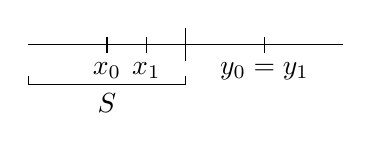
\begin{tikzpicture}
  \draw (-2,0) to (2,0);
  \draw (-1,3pt) to (-1,-3pt) node[anchor=north] {\( x_{0} \)};
  \draw ({-1/2},3pt) to ({-1/2},-3pt) node[anchor=north] {\( x_{1} \)};
  \draw (0,6pt) to (0,-6pt);
  \draw (1,3pt) to (1,-3pt) node[anchor=north] {\( y_{0}=y_{1} \)};
  \draw (-2,-0.4) to (-2,-0.5) to (0,-0.5) to (0,-0.4);
  \node[anchor=north] at (-1,-0.5) {\( S \)};
\end{tikzpicture}
Two options exist: if \(m_{0}\) is an upper bound for \(S\), set \(y_{1}=m_{0}\) and \(x_{1}=x_{0}\).\\[0pt]
Otherwise, \(\exists x_{1}\in S\), such that \(m_{0}<x_{1}\) so set \(y_{1}=y_{0}\).\\[0pt]
Repeat this process forever to construct two sequences \(x_{n},\;y_{n}\).\\[0pt]
\(\forall n,\;x_{n}\in S\), \(y_{n}\) is an upper bound for \(S\).\\[0pt]
\begin{itemize}
\item \(x_{n}\leq y_{n}\)\\[0pt]
\item \(x_{n}\) is increasing and bounded above by \(y_{0}\), so it must be Cauchy and converging to \(x\).\\[0pt]
\item \(y_{n}\) is decreasing and bounded below by \(x_{0}\), so it must be Cauchy and converging to \(y\).\\[0pt]
\item \(|x_{n+1}-y_{n+1}|\leq\frac{|x_{n}-y_{n}|}{2}\) which implies \(|x_{n}-y_{n}|\leq\frac{1}{2^{n}}|x_{0}-y_{0}|\) and \(x=y=z\).\\[0pt]
\end{itemize}
Therefore, the process may be understood as \(x_{0}\leq\cdots\leq x_{n}\leq x_{n+1}\leq y_{n+1}\leq y_{n}\leq\cdots\leq y_{0}\).\\[0pt]
There remain two things to check: (1) \(z\) is an upper bound for \(S\) and (2) \(z\) is no larger than any other upper bound for \(S\).\\[0pt]
\begin{enumerate}
\item Take \(x\in S,\;\forall n,\;x\leq y_{n}\overset{n\to\infty}{\longrightarrow}x\leq Z\).\\[0pt]
\item Take upper bound for \(S\), \(z'\). \(x_{n}\leq z',\;\forall n\overset{n\to\infty}{\longrightarrow}z\leq z'\).\\[0pt]
\end{enumerate}
So \(z=\sup{S}\).\\[0pt]
\subsection*{Monotone Convergence Theorem (Completeness 3)}
\label{sec:orgee99e53}
An increasing sequence of reals, \(\{x_{n}\}_{n}\), that is bounded above, converges to \(\sup{X}=\sup\{x_{n}|n\in\N\}\).\\[0pt]
To prove that this converges, since it is monotone and bounded above it is Cauchy and therefore must be convergent.\\[0pt]
\subsubsection*{Proof}
\label{sec:org0684715}
Call \(x\) the limit, then \(\forall n,\;x_{n}\leq x\). To see this, suppose \(\exists n_{0},\;x<x_{n_{0}}\) then \(\forall m\geq m_{0},\;x<x_{m_{0}}\leq x_{m} \implies |x_{m}-x|\geq|x_{n_{0}}-x|>0,\;\forall m\geq n_{0}\) is a contradiction.\\[0pt]
Let \(M\) be an upper bound of \(X\). Then \(x_{n}\leq M,\;\forall n\overset{n\to\infty}{\longrightarrow}x\leq M\implies x=\sup{X}\).\\[0pt]
\subsection*{Theorem (Existence of Roots)}
\label{sec:org5391460}
\(\forall x\in\R\) where \(x>0,\;p\in\{2,3,\;\ldots\;,\},\;\exists!y>0\) such that \(y^{p}=x\).\\[0pt]
\subsubsection*{Proof}
\label{sec:org44f4ca7}
Left as an exercise.\\[0pt]
Either by dichotomy or consider \(S=\{y\in\R|y^{p}<x\}\), show: \(S\neq 0\), bounded above and \((\sup{S})^{p}=x\).\\[0pt]
For uniqueness, show \(y_{1}^{p}=y_{2}^{p}=x \iff 0=y_{1}^{p}-y_{2}^{p}=(y_{1}-y_{2})(\cdots\neq 0)\implies y_{1}=y_{2}\).\\[0pt]
\subsection*{Topological Properties}
\label{sec:org308a43d}
\(S\subseteq\R\) is open if \(\forall x\in S,\;\exists a,b\in\R,\;x\in(a,b)\subset S\).\\[0pt]
\(x\) is an accumulation or limit point of \(S\) if \(\forall\epsilon>0,\;\exists y\in S,\;|0<|x-y|<\epsilon\).\\[0pt]
\(S\subseteq\R\) is closed if it contains all its limit points.\\[0pt]
A set may be both open closed, just open, just closed or neither.\\[0pt]
Given \(S\subseteq\R\), the interior of \(S\) is \(\bigcup_{S'\text{ open}\subset S}S'=S^{\text{int}}=S^{0}\).\\[0pt]
The closure is \(\bigcap_{F\text{ closed}\supseteq S}F=\overline{S}\overset{\text{wts}}{=}S\cup\{\text{limit points of }S\}\).\\[0pt]
\subsubsection*{Example}
\label{sec:org4668b20}
\(\{x\}\) is not open, but, since the limit points of \(x\) are \(\0\), it is closed.\\[0pt]
\subsubsection*{Propositions}
\label{sec:org05753cb}
\begin{enumerate}
\item Arbitrary unions and finite intersections of open sets are open.\\[0pt]
\item \(S\) is open if and only the complement \(S^{c}=\R\setminus S\) is closed.\\[0pt]
\item Arbitrary intersections and finite unions of closed sets are closed.\\[0pt]
\end{enumerate}
\subsection*{Bolzano-Weierstrass Theorem}
\label{sec:orgbb27dff}
A bounded sequence in \(\R\) ad mits a convergent (Cauchy) subsequence. \(\exists M,\;|x_{n}|\leq M,\;\forall n\)\\[0pt]
\subsubsection*{Proof by Dichotomy}
\label{sec:org5bee109}
Suppose \(I_{0}=[a,b]\) contains the sequence.\\[0pt]
Construct a sequence of intervals by indicators: if \(\left[ a,\frac{a+b}{2} \right]\) contains infinitely terms of \(\{x_{n}\}_{n}\), choose \(n\) such that \(x_{n_{1}}\in\left[ a,\frac{a+b}{2} \right]\) and call \(I_{1}=\left[ a,\frac{a+b}{2} \right]\).\\[0pt]
Otherwise, \(\left[ \frac{a+b}{2},b \right]\) must contain infinitely many terms. Choose \(n\) in a similar fashion as above such that \(I_{1}=\left[ \frac{a+b}{2},b \right]\).\\[0pt]
This process may be repeated to create a sequence of intervals such that \(I_{k}\supseteq I_{k+1}\supseteq I_{k+2}\) and \(l(I_{k})=\frac{b-a}{2^{k}}\).\\[0pt]
A subsequence \(\{u_{n_{k}}\}_{k}\) such that \(u_{n_{k}}\in I_{l}\) for \(k\geq l\).\\[0pt]
\subsubsection*{Exercise}
\label{sec:org9f668c3}
Extract a Cauchy criterion out of the above.\\[0pt]
\end{document}